\begin{figure*}[h!t]
    \centering
    %
    \resizebox{0.6\textwidth}{!}{
        
\begin{tikzpicture}[scale=1.0, every node/.style={scale=1.0}]
            \draw[thick, black] (-3, -0.25) rectangle (10, 0.25);
            %
            \draw[black, line width=1pt] (-2.5, 0.0) -- (-2,0.0);
            \fill[black] (-2.25,0.0) circle (2pt); %
            \node[right] at (-2,0.0) {\small Observed Path};
            
            %
            \draw[blue, line width=1pt] (1.0,0.0) -- (1.5,0.0);
            \node[draw=blue, circle, minimum size=4pt, inner sep=0pt] at (1.25,0.0) {}; %
            \node[right] at (1.5,0.0) {\small Interval CFMDP Policy};
            
            %
            \draw[red, line width=1pt] (5.5,0) -- (6,0);
            \node[red] at (5.75,0) {$\boldsymbol{\times}$}; %
            \node[right] at (6,0) {\small Gumbel-max SCM Policy};
        \end{tikzpicture}
    }\\
    \subfigure[\footnotesize Lowest cumulative reward: Interval CFMDP ($415$), Gumbel-max SCM ($415$)]{%
         \resizebox{0.76\columnwidth}{!}{
             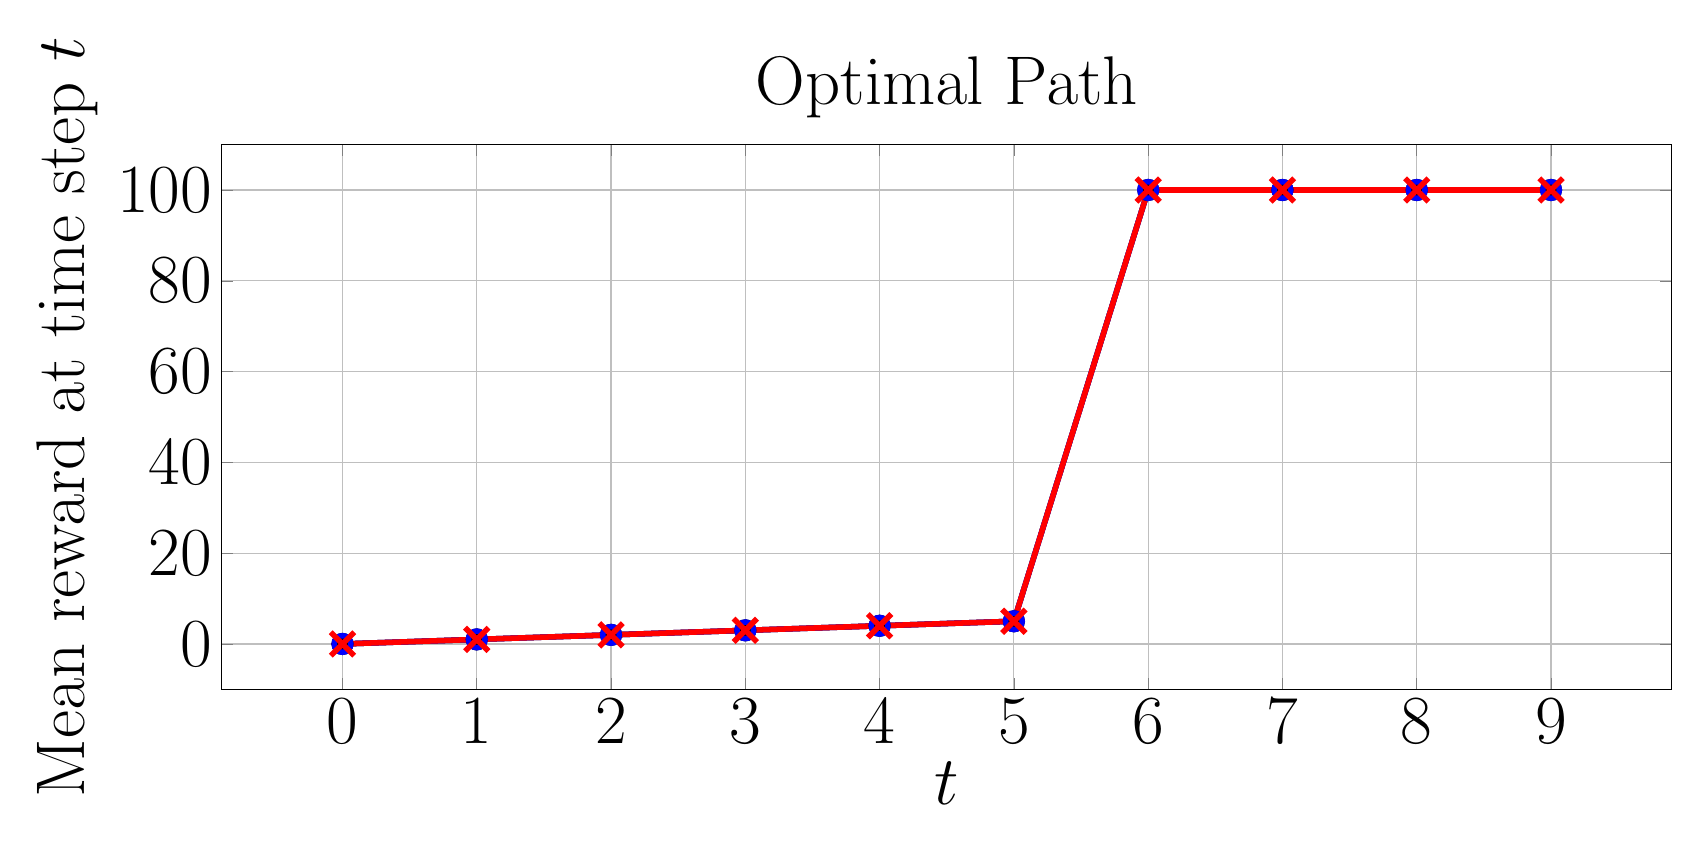
\begin{tikzpicture}
                 \begin{axis}[
                        xlabel={$t$},
                        ylabel={Mean reward at time step $t$},
                        title={Optimal Path},
                        every axis/.style={font=\Huge},
                        grid=both,
                        width=20cm, height=8.5cm,
                        %
                ]
                \addplot[
                    color=black, %
                    mark=*, %
                    line width=2pt,
                    mark size=3pt,
                ]
                coordinates {
                    (0, 0.0)
                    (1, 1.0)
                    (2, 2.0)
                    (3, 3.0)
                    (4, 4.0)
                    (5, 5.0)
                    (6, 100.0)
                    (7, 100.0)
                    (8, 100.0)
                    (9, 100.0)
                };
                \addplot[
                    color=blue, %
                    mark=o, %
                    line width=2pt,
                    mark size=3pt,
                    error bars/.cd,
                    y dir=both, %
                    y explicit, %
                    error bar style={line width=1pt,solid},
                    error mark options={line width=1pt,mark size=4pt,rotate=90}
                ]
                 coordinates {
                    (0, 0.0)  +- (0, 0.0)
                    (1, 1.0)  +- (0, 0.0) 
                    (2, 2.0)  +- (0, 0.0) 
                    (3, 3.0)  +- (0, 0.0)
                    (4, 4.0)  +- (0, 0.0)
                    (5, 5.0) +- (0, 0.0)
                    (6, 100.0) +- (0, 0.0)
                    (7, 100.0) +- (0, 0.0)
                    (8, 100.0) +- (0, 0.0)
                    (9, 100.0) +- (0, 0.0)
                };
                \addplot[
                    color=red, %
                    mark=x, %
                    line width=2pt,
                    mark size=6pt,
                    error bars/.cd,
                    y dir=both, %
                    y explicit, %
                    error bar style={line width=1pt,solid},
                    error mark options={line width=1pt,mark size=4pt,rotate=90}
                ]
                 coordinates {
                    (0, 0.0)  +- (0, 0.0)
                    (1, 1.0)  +- (0, 0.0) 
                    (2, 2.0)  +- (0, 0.0) 
                    (3, 3.0)  +- (0, 0.0)
                    (4, 4.0)  +- (0, 0.0)
                    (5, 5.0) +- (0, 0.0)
                    (6, 100.0) +- (0, 0.0)
                    (7, 100.0) +- (0, 0.0)
                    (8, 100.0) +- (0, 0.0)
                    (9, 100.0) +- (0, 0.0)
                };
                %
                %
                %
                %
                %
                %
                %
                %
                %
                %
                %
                %
                %
                %
                %
                %
                %
                %
                %
                %
                %
                \end{axis}
             \end{tikzpicture}
         }
    }
    \hspace{1cm}
    \subfigure[\footnotesize Lowest cumulative reward: Interval CFMDP ($-495$), Gumbel-max SCM ($-495$)]{%
         \resizebox{0.76\columnwidth}{!}{
            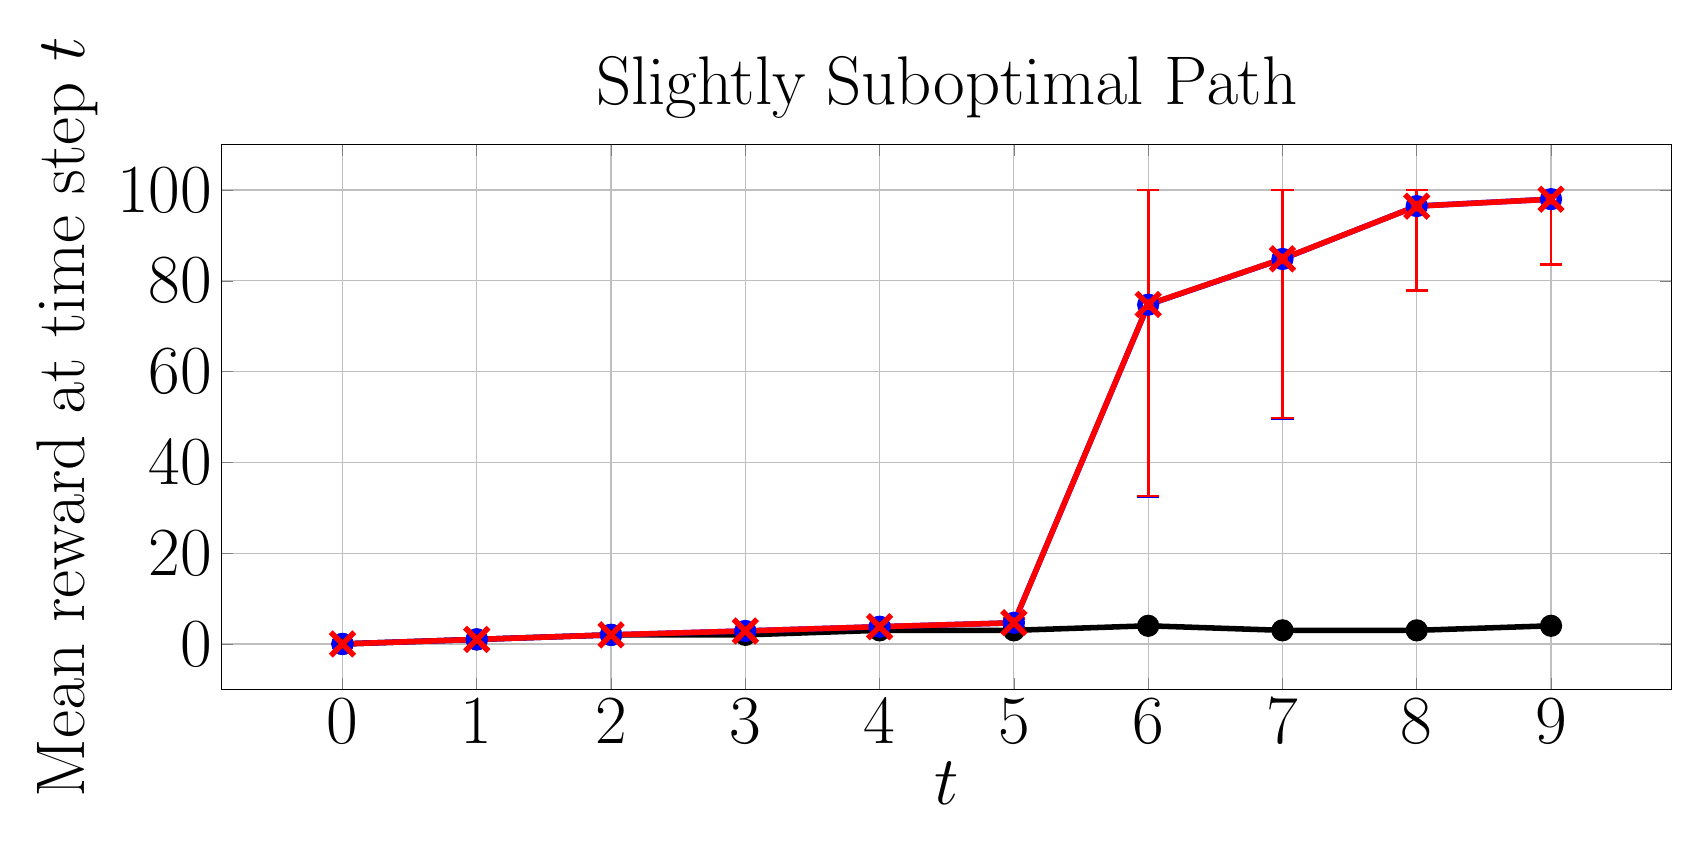
\begin{tikzpicture}
                \begin{axis}[
                    xlabel={$t$},
                    ylabel={Mean reward at time step $t$},
                    title={Slightly Suboptimal Path},
                    every axis/.style={font=\Huge},
                    grid=both,
                    width=20cm, height=8.5cm,
                    %
                ]
                \addplot[
                    color=black, %
                    mark=*, %
                    line width=2pt,
                    mark size=3pt,
                ]
                coordinates {
                    (0, 0.0)
                    (1, 1.0)
                    (2, 2.0)
                    (3, 2.0)
                    (4, 3.0)
                    (5, 3.0)
                    (6, 4.0)
                    (7, 3.0)
                    (8, 3.0)
                    (9, 4.0)
                };
                %
               \addplot[
                    color=blue, %
                    mark=o, %
                    line width=2pt,
                    mark size=3pt,
                    error bars/.cd,
                    y dir=both, %
                    y explicit, %
                    error bar style={line width=1pt,solid},
                    error mark options={line width=1pt,mark size=4pt,rotate=90}
                ]
                coordinates {
                (0, 0.0)  +- (0, 0.0)
                (1, 1.0)  +- (0, 0.0)
                (2, 2.0)  +- (0, 0.0)
                (3, 2.8661345)  +- (0, 0.42603466)
                (4, 3.798614)  +- (0, 0.52865932)
                (5, 4.6613305)  +- (0, 1.02983565)
                (6, 74.7305995) += (0, 25.2694005) -= (0, 42.20242079)
                (7, 84.802457)  += (0, 15.197543)  -= (0, 35.08575705)
                (8, 96.455942)  += (0, 3.544058)   -= (0, 18.4617318)
                (9, 97.9790975) += (0, 2.0209025)  -= (0, 14.29029466)
            };
                %
                \addplot[
                    color=red, %
                    mark=x, %
                    line width=2pt,
                    mark size=6pt,
                    error bars/.cd,
                    y dir=both, %
                    y explicit, %
                    error bar style={line width=1pt,solid},
                    error mark options={line width=1pt,mark size=4pt,rotate=90}
                ]
                coordinates {
                (0, 0.0)  +- (0, 0.0)
                (1, 1.0)  +- (0, 0.0)
                (2, 2.0)  +- (0, 0.0)
                (3, 2.866351)  +- (0, 0.42523987)
                (4, 3.799144)  +- (0, 0.52810308)
                (5, 4.662749)  +- (0, 1.00452614)
                (6, 74.773081) += (0, 25.226919)   -= (0, 42.17816553)
                (7, 84.833464) += (0, 15.166536)   -= (0, 35.06110031)
                (8, 96.4349945) += (0, 3.5650055)  -= (0, 18.51953372)
                (9, 97.9669475) += (0, 2.0330525)  -= (0, 14.33075378)
            };
                %
               %
               %
               %
               %
               %
               %
               %
               %
               %
               %
               %
               %
               %
               %
               %
               %
               %
               %
                \end{axis}
            \end{tikzpicture}
         }
    }\\[-1.5pt]
    \subfigure[\footnotesize Lowest cumulative reward: Interval CFMDP ($-697$), Gumbel-max SCM ($-698$)]{%
         \resizebox{0.76\columnwidth}{!}{
             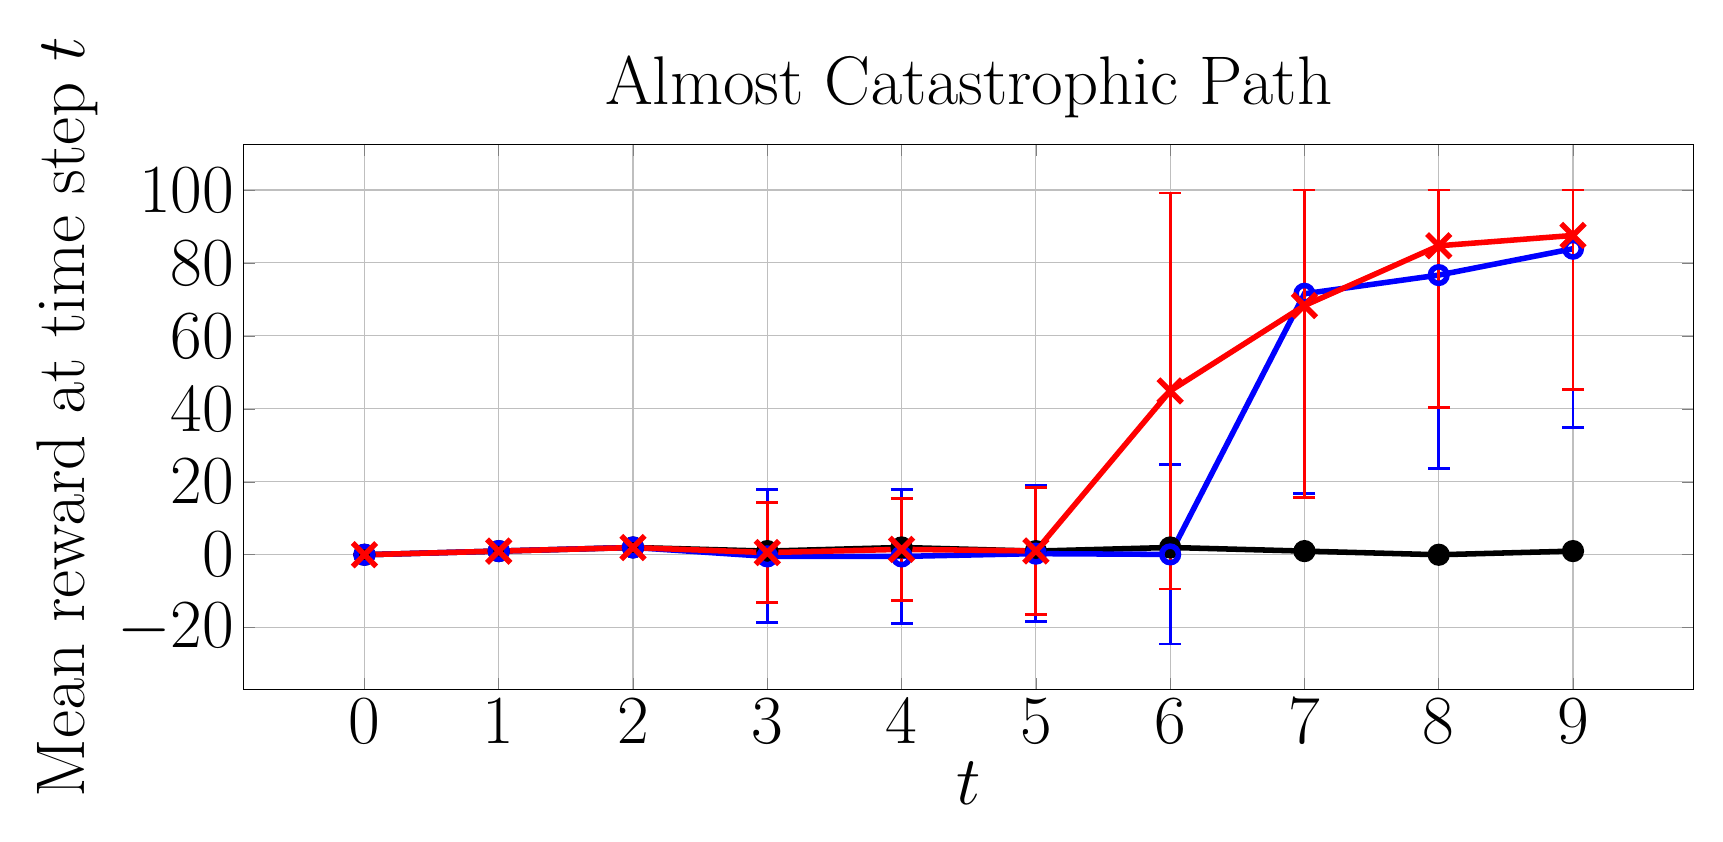
\begin{tikzpicture}
                \begin{axis}[
                    xlabel={$t$},
                    ylabel={Mean reward at time step $t$},
                    title={Almost Catastrophic Path},
                    every axis/.style={font=\Huge},
                    grid=both,
                    width=20cm, height=8.5cm,
                    %
                ]
                \addplot[
                    color=black, %
                    mark=*, %
                    line width=2pt,
                    mark size=3pt,
                ]
                coordinates {
                    (0, 0.0)
                    (1, 1.0)
                    (2, 2.0)
                    (3, 1.0)
                    (4, 2.0)
                    (5, 1.0)
                    (6, 2.0)
                    (7, 1.0)
                    (8, 0.0)
                    (9, 1.0)
                };
                %
                \addplot[
                    color=blue, %
                    mark=o, %
                    line width=2pt,
                    mark size=3pt,
                    error bars/.cd,
                    y dir=both, %
                    y explicit, %
                    error bar style={line width=1pt,solid},
                    error mark options={line width=1pt,mark size=4pt,rotate=90}
                ]
                coordinates {
                    (0, 0.0)  +- (0, 0.0)
                    (1, 1.0)  +- (0, 0.0)
                    (2, 2.0)  +- (0, 0.0)
                    (3, -0.445837)  +- (0, 18.2323085)
                    (4, -0.4585655)  +- (0, 18.40684148)
                    (5, 0.3053175)  +- (0, 18.62866744)
                    (6, 0.0956245)  +- (0, 24.55051607)
                    (7, 71.54727)  += (0, 28.45273)   -= (0, 54.83199135)
                    (8, 76.670842) += (0, 23.329158)  -= (0, 52.9386188)
                    (9, 83.902088) += (0, 16.097912)  -= (0, 49.00201108)
                };
                %
                \addplot[
                    color=red, %
                    mark=x, %
                    line width=2pt,
                    mark size=6pt,
                    error bars/.cd,
                    y dir=both, %
                    y explicit, %
                    error bar style={line width=1pt,solid},
                    error mark options={line width=1pt,mark size=4pt,rotate=90}
                ]
                coordinates {
                (0, 0.0)  +- (0, 0.0)
                (1, 1.0)  +- (0, 0.0)
                (2, 1.96988)  +- (0, 0.21136647)
                (3, 0.602197)  +- (0, 13.77136924)
                (4, 1.4765265)  +- (0, 14.02177032)
                (5, 1.0409715)  +- (0, 17.50019462)
                (6, 44.898029)  +- (0, 54.28467191)
                (7, 68.319994)  += (0, 31.680006) -= (0, 52.5192166)
                (8, 84.6988915) += (0, 15.3011085) -= (0, 44.36762745)
                (9, 87.540126)  += (0, 12.459874)  -= (0, 42.13634702)
            };
                %
               %
               %
               %
               %
               %
               %
               %
               %
               %
               %
               %
               %
               %
               %
               %
               %
               %
               %
                \end{axis}
            \end{tikzpicture}
         }
    }
    \hspace{1cm}
    \subfigure[\footnotesize Lowest cumulative reward: Interval CFMDP ($-698$), Gumbel-max SCM ($-698$)]{%
         \resizebox{0.76\columnwidth}{!}{
            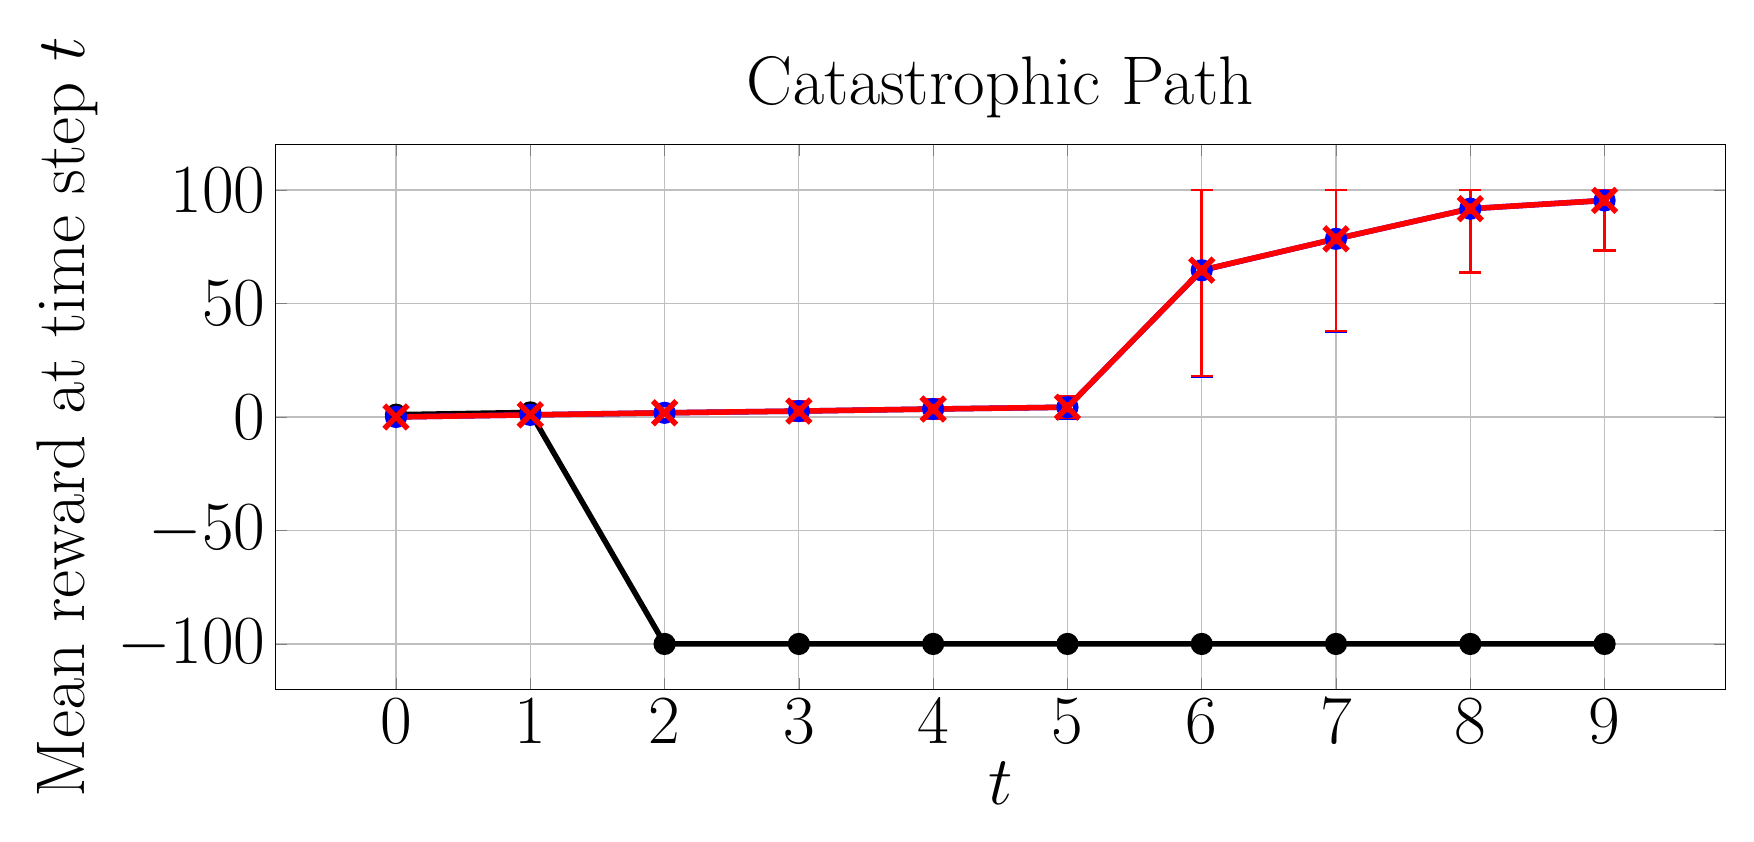
\begin{tikzpicture}
                \begin{axis}[
                    xlabel={$t$},
                    ylabel={Mean reward at time step $t$},
                    title={Catastrophic Path},
                    every axis/.style={font=\Huge},
                    grid=both,
                    width=20cm, height=8.5cm,
                    %
                ]
                \addplot[
                    color=black, %
                    mark=*, %
                    line width=2pt,
                    mark size=3pt,
                ]
                coordinates {
                    (0, 1.0)
                    (1, 2.0)
                    (2, -100.0)
                    (3, -100.0)
                    (4, -100.0)
                    (5, -100.0)
                    (6, -100.0)
                    (7, -100.0)
                    (8, -100.0)
                    (9, -100.0)
                };
                %
                \addplot[
                    color=blue, %
                    mark=o, %
                    line width=2pt,
                    mark size=3pt,
                    error bars/.cd,
                    y dir=both, %
                    y explicit, %
                    error bar style={line width=1pt,solid},
                    error mark options={line width=1pt,mark size=4pt,rotate=90}
                ]
                coordinates {
                (0, 0.0)  +- (0, 0.0)
                (1, 0.934776)  +- (0, 0.2469207) 
                (2, 1.836178)  +- (0, 0.41747018) 
                (3, 2.589682)  +- (0, 4.25205246)
                (4, 3.498908)  +- (0, 4.43656509)
                (5, 4.294412)  +- (0, 4.79783311)
                (6, 64.6238925) += (0, 35.3761075) -= (0, 46.69660801)
                (7, 78.4716035) += (0, 21.5283965) -= (0, 40.66803792)
                (8, 91.745166)  += (0, 8.254834)  -= (0, 28.04970295)
                (9, 95.393843)  += (0, 4.606157)  -= (0, 22.08917601)
                };
                %
                \addplot[
                    color=red, %
                    mark=x, %
                    line width=2pt,
                    mark size=6pt,
                    error bars/.cd,
                    y dir=both, %
                    y explicit, %
                    error bar style={line width=1pt,solid},
                    error mark options={line width=1pt,mark size=4pt,rotate=90}
                ]
                coordinates {
                    (0, 0.0)  +- (0, 0.0)
                    (1, 0.934791)  +- (0, 0.24689428)
                    (2, 1.8360415)  +- (0, 0.41772372)
                    (3, 2.596742)  +- (0, 4.16891772)
                    (4, 3.503747)  +- (0, 4.38250693)
                    (5, 4.300445)  +- (0, 4.74124465)
                    (6, 64.6758075) += (0, 35.3241925) -= (0, 46.67192883)
                    (7, 78.483407)  += (0, 21.516593)  -= (0, 40.64493202)
                    (8, 91.75123)   += (0, 8.24877)    -= (0, 28.02106014)
                    (9, 95.407927)  += (0, 4.592073)   -= (0, 22.05066531)
                };
                %
               %
               %
               %
               %
               %
               %
               %
               %
               %
               %
               %
               %
               %
               %
               %
               %
               %
               %
                \end{axis}
            \end{tikzpicture}
         }
    }
\caption{Average instant reward of CF paths induced by policies on GridWorld $p=0.9$. Error bars denote the standard deviation in reward at each time step, and below each graph, we note the lowest cumulative reward across all counterfactual paths induced by each policy.}
\label{fig: reward p=0.9}
\end{figure*}

\section{Methodology}
With our analytical bounds, we can compute a non-stationary interval counterfactual MDP for any MDP $\mathcal{M}$ and observed path $\tau$. Formally, an interval Markov decision process (IMDP) \citep{GIVAN200071} is a tuple $(\mathcal{S}, \mathcal{A}, P_{\updownarrow}, \mathcal{R})$, extending MDPs with an uncertain transition probability function $P_{\updownarrow}$ that maps each transition to a probability within its bounds $P_{\updownarrow}(s' \mid s, a) = [P^{\it LB}(s' \mid s, a), P^{\it UB}(s' \mid s, a)]$. To construct an interval counterfactual MDP, we compute the counterfactual probability bounds for every transition in the MDP, given every observed transition in $\tau$.
\begin{definition}[Interval Counterfactual MDP (ICFMDP)]
Given an observed path $\tau$ and MDP $\mathcal{M}$, the counterfactual probability for each transition in the interval counterfactual MDP (ICFMDP) ${\tilde{\mathcal{M}}^{\updownarrow}_{\tau}}$ is defined, for $t=0,\ldots,T-1$, as $\tilde{P}^{\updownarrow}_{t}(\tilde{s}' \mid \tilde{s}, \tilde{a}) = [\tilde{P}_{t}^{\it LB}(\tilde{s'} \mid \tilde{s}, \tilde{a}), \tilde{P}_{t}^{\it UB}(\tilde{s'} \mid \tilde{s}, \tilde{a})]$.
%
%
%
%
%
%
\end{definition}
\jl{To derive optimal counterfactual policies for this ICFMDP, we apply robust value iteration  \citep{mathiesen2024intervalmdp}, which pessimistically optimises the expected reward 
$$V^{*}(s) = \max_{\pi} \min_{\tilde{P}_t \in \tilde{P}^{\updownarrow}_{t}}\mathbb{E}_{s' \sim \tilde{P}_t(\cdot \mid s, \pi(s))}\left[R(s, \pi(s)) + V^{*}(s')\right].$$ In Appendix \ref{sec: sampled interval cfmdp proof}, we prove that any CFMDP entailed by the ICFMDP will be valid (i.e., satisfying \eqref{eq: optimisation} + \eqref{eq: additional assumptions}), \jl{so this policy will be robust across all possible causal models (i.e., the ICFMDP does not introduce spurious models).}}
%
%
%

%
%
%
%
